%%% Realisering af optimering af udgangsfilter %%%

\subsection{Udgangsfilter}
I dette afsnit testes udgangssignalet, efter udgangen er blevet flyttet. På figur~\ref{fig:realisering_udgang_f_filter_3} ses udgangssignalet målt før filteret. Her ses det, at spikes'ene er blevet ift. ved 2. iteration. Dette komme ved den hurtigere switch-tid i MOSFET'en, der skaber større transient-peaks. Dette understreger nødvendigheden for funktionaliteten i udgangsfilteret.

\begin{figure}[H]
	\center
	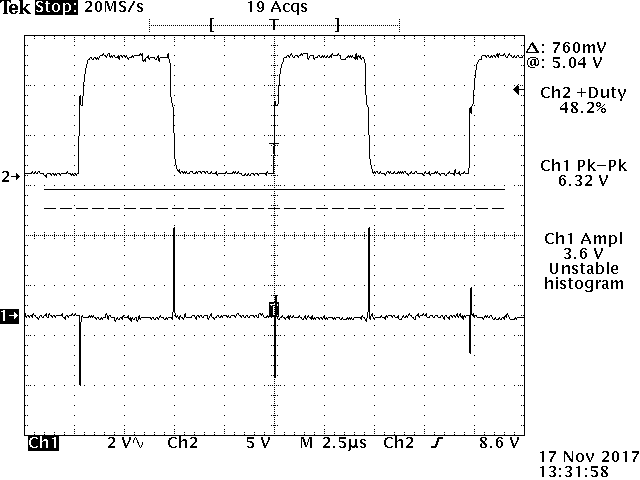
\includegraphics[max width=0.7\linewidth]{/tex/3iteration/billeder/Realisering/Output_26V.png}
	\caption{Udgangssignal før filter - 3. iteration}
	\label{fig:realisering_udgang_f_filter_3}
\end{figure}

\noindent Figur~\ref{fig:realisering_udgang_e_filter_3} viser udgangssignalet efter filteret. Her ses det spikes'ene er blevet dæmpet til en pk-pk på $920mV$. Dette viser tydeligt der er opnået en dæmpning af switching-spikes ved bare, at flytte udgangen. Det er dog ikke nok ift. kravet på $100mV$ pk-pk. Derfor skal dette optimeres yderligere i en senere iteration.

\begin{figure}[H]
	\center
	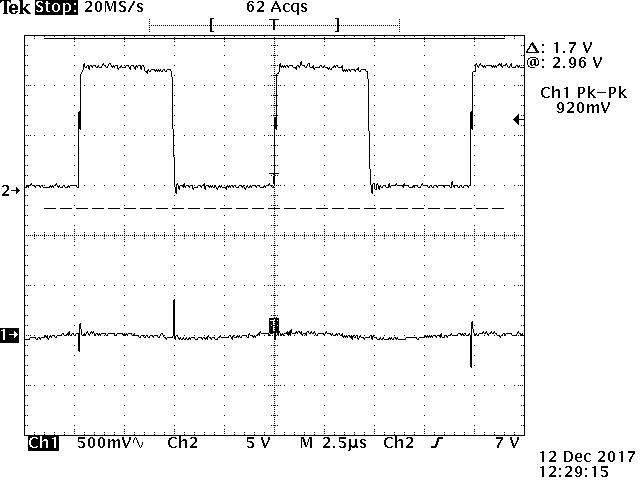
\includegraphics[max width=0.7\linewidth]{/tex/3iteration/billeder/Realisering/udgang_e_filter_3iteration.png}
	\caption{Udgangssignal efter filter - 3. iteration}
	\label{fig:realisering_udgang_e_filter_3}
\end{figure}

\noindent Figur~\ref{fig:realisering_udgang_e_filter_zoom_3} viser et zoom af udgangsspændingen, for at tydeliggøre ripplespændingen. Den aflæses til ca. $50mV$, hvilket er det ønskede niveau. 

\begin{figure}[H]
	\center
	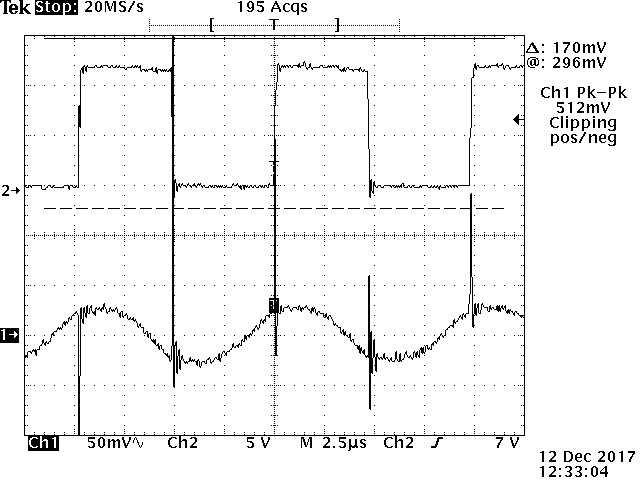
\includegraphics[max width=0.7\linewidth]{/tex/3iteration/billeder/Realisering/udgang_e_filter_3iteration_zoom.png}
	\caption{Udgangsripple - 3. iteration}
	\label{fig:realisering_udgang_e_filter_zoom_3}
\end{figure}